El ransomware puede ser categorizado en tres formas principales: locker, cripto y scareware\autocite{beaman2021ransomware}:

\begin{figure}[H]
\centering
\usetikzlibrary{positioning, arrows.meta, shapes, backgrounds}


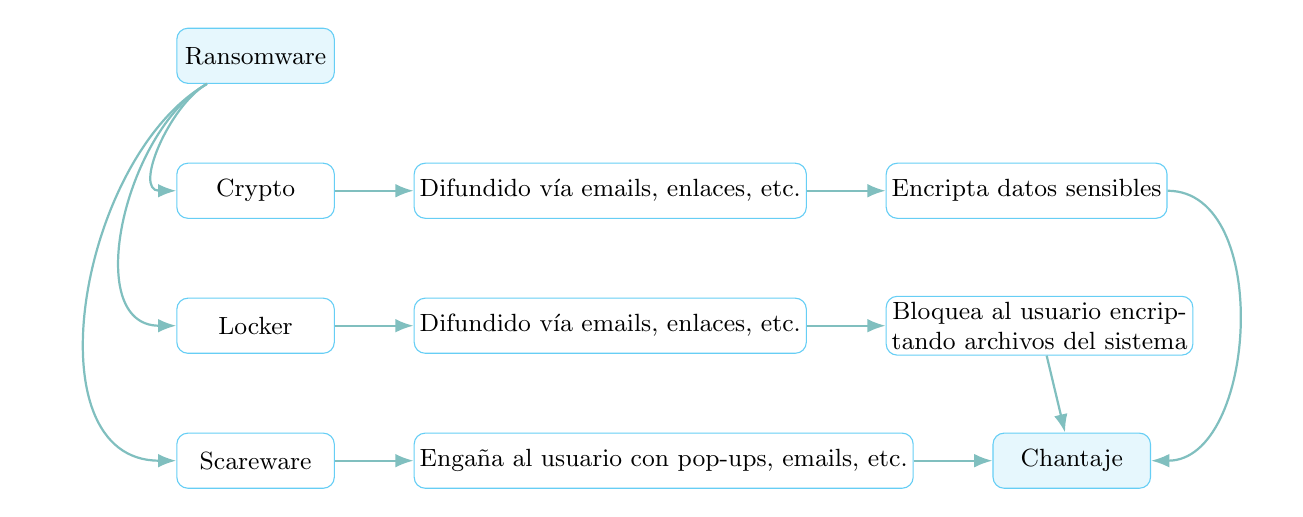
\begin{tikzpicture}[
    nodo/.style={
        rectangle,
        rounded corners,
        draw=cyan!60,
        align=center,
        fill=white, % color de fondo predeterminado
        font=\small,
        inner sep=2pt,
        minimum width=2cm,
        minimum height=0.7cm,
    },
    nodo_coloreado/.style={nodo, fill=cyan!10}, % nuevo estilo para nodos coloreados
    arr/.style={-Latex, thick,, draw=teal!50}
]

% Nodos
\node[nodo_coloreado] (ransomware) {Ransomware}; % nodo coloreado
\node[nodo, below=of ransomware] (crypto) {Crypto};
\node[nodo, below=of crypto] (locker) {Locker};
\node[nodo, below=of locker] (scareware) {Scareware};
\node[nodo, right=of crypto] (emailscrypto) {Difundido vía emails, enlaces, etc.};
\node[nodo, right=of locker] (emailslocker) {Difundido vía emails, enlaces, etc.};
\node[nodo, right=of scareware] (popupsscare) {Engaña al usuario con pop-ups, emails, etc.};
\node[nodo, right=of emailscrypto] (encryptdata) {Encripta datos sensibles};
\node[nodo, right=of emailslocker] (lockout) {Bloquea al usuario encrip-\\tando archivos del sistema};
\node[nodo_coloreado, right=of popupsscare] (blackmail) {Chantaje}; % nodo coloreado

% Conexiones principales
\draw[arr] (ransomware) edge[arr, out=210, in=180]   (crypto.west);
\draw[arr] (ransomware) edge[arr, out=210, in=180] (locker.west);
\draw[arr] (ransomware) edge[arr, out=210, in=180] (scareware.west);

\draw[arr] (crypto) -- (emailscrypto);
\draw[arr] (locker) -- (emailslocker);
\draw[arr] (scareware) -- (popupsscare);

% Conexiones a nodos de acción
\draw[arr] (emailscrypto) -- (encryptdata);
\draw[arr] (emailslocker) -- (lockout);
\draw[arr] (popupsscare) -- (blackmail);

% Ajustes a las conexiones para evitar cruce usando el método 'edge'
\path (encryptdata.east) edge[arr, out=0, in=0] (blackmail.east);
\path (lockout) edge[arr] (blackmail);

\end{tikzpicture}


\caption{Tipos de Ransomware y sus métodos de difusión.}
\end{figure}

\subsubsection{Locker ransomware}
El ransomware tipo locker puede cifrar archivos específicos, lo que puede resultar en el bloqueo de la pantalla y/o el teclado del ordenador.

Sin embargo, generalmente es fácil de superar y, frecuentemente, se puede resolver reiniciando el sistema en modo seguro o ejecutando un escáner de virus bajo demanda.

\subsubsection{Crypto Ransomware}
Este es el tipo más común y peligroso de ransomware. Utiliza algoritmos de cifrado para bloquear el acceso a archivos y documentos importantes en el sistema de la víctima. Puede utilizar uno de tres esquemas de cifrado .
\begin{itemize}
    \item Simétrico. El enfoque de cifrado simétrico en el ransomware implica utilizar una única clave para cifrar y descifrar los datos. Esta clave se comparte entre el atacante y la víctima.
    \item Asimétrico. Implica el uso de un par de claves: una pública y otra privada. La clave pública se utiliza para cifrar los datos, mientras que la clave privada correspondiente se utiliza para descifrarlos.
    \item Híbrido. Combina cifrado simétrico y asimétrico para cifrar los archivos de la víctima, utilizando una clave generada por el ransomware que luego se cifra con una clave pública desde un servidor C\&C, haciendo que el descifrado dependa de obtener la clave privada tras pagar un rescate.
\end{itemize}

\subsubsection{Scareware}
El scareware se basa en tácticas de manipulación psicológica. Se utilizan mensajes intimidantes que sugieren que el dispositivo ha sido comprometido por virus o malware, para que el usuario pague para eliminar la supuesta amenaza. Estos mensajes pueden aparecer en forma de pop-ups, mensajes emergentes o correos electrónicos falsos. Esta modalidad de ransomware no causa daños directos al sistema informático de la víctima, no cifra los datos ni bloquea el dispositivo. 